\section{Actions In Combat}
Here are the fundamental actions for moving, attacking, casting spells, and manifesting powers. More specialized options are covered by the sections Special Attacks and Special Initiative Actions.

\subsection{The Combat Round}
Each round represents 6 seconds in the game world. A round presents an opportunity for each character involved in a combat situation to take an action.

Each round's activity begins with the character with the highest initiative result and then proceeds, in order, from there. Each round of a combat uses the same initiative order. When a character's turn comes up in the initiative sequence, that character performs his entire round's worth of actions. (For exceptions, see Attacks of Opportunity and Special Initiative Actions.)

For almost all purposes, there is no relevance to the end of a round or the beginning of a round. A round can be a segment of game time starting with the first character to act and ending with the last, but it usually means a span of time from one round to the same initiative count in the next round. Effects that last a certain number of rounds end just before the same initiative count that they began on.


\subsection{Action Types}
An action's type essentially tells you how long the action takes to perform (within the framework of the 6-second combat round) and how movement is treated. There are six types of actions: standard actions, move actions, full-round actions, free actions, swift actions, and immediate actions.

In a normal round, you can perform a standard action and a move action, or you can perform a full-round action. You can also perform one or more free actions. You can always take a move action in place of a standard action.

In some situations (such as in a surprise round), you may be limited to taking only a single move action or standard action.

\textbf{Standard Action:} A standard action allows you to do something, most commonly make an attack or cast a spell. See Table: Standard Actions for other standard actions.

\textbf{Move Action:} A move action allows you to move your speed or perform an action that takes a similar amount of time. See Table: Move Actions.

You can take a move action in place of a standard action. If you move no actual distance in a round (commonly because you have swapped your move for one or more equivalent actions), you can take one 5-foot step either before, during, or after the action.

\textbf{Full-Round Action:} A full-round action consumes all your effort during a round. The only movement you can take during a full-round action is a 5-foot step before, during, or after the action. You can also perform free actions (see below).

Some full-round actions do not allow you to take a 5-foot step.

Some full-round actions can be taken as standard actions, but only in situations when you are limited to performing only a standard action during your round. The descriptions of specific actions, below, detail which actions allow this option.

\textbf{Free Action:} Free actions consume a very small amount of time and effort. You can perform one or more free actions while taking another action normally. However, there are reasonable limits on what you can really do for free.

\textbf{Swift Action:} A swift action consumes a very small amount of time, but represents a larger expenditure of effort and energy than a free action. You can perform only a single swift action per turn.

\textbf{Immediate Action:} An immediate action is very similar to a swift action, but can be performed at any time---even if it's not your turn.

\textbf{Not an Action:} Some activities are so minor that they are not even considered free actions. They literally don't take any time at all to do and are considered an inherent part of doing something else.

\textbf{Restricted Activity:} In some situations, you may be unable to take a full round's worth of actions. In such cases, you are restricted to taking only a single standard action or a single move action (plus free actions as normal). You can't take a full-round action (though you can start or complete a full-round action by using a standard action; see below).
\Figure*{t}{images/monk-1.png}
\subsection{Standard Actions}

\Table{Standard Actions}{LZ{14mm}}{
\tableheader Action & \tableheader Attack of Opportunity\footnotemark[1]\\
Attack (melee) & No\\
Attack (unarmed) & Yes\\
Attack (ranged) & Yes\\
Activate a magic item other than a potion or oil & No\\
Activate a psionic tattoo & Yes\\
Aid another & Maybe\footnotemark[2]\\
Bull rush & Yes\\
Cast a spell (1 standard action casting time) & Yes\\
Concentrate to maintain an active spell & No\\
Concentrate to maintain an active power & No\\
Dismiss a spell & No\\
Dismiss a power & No\\
Draw a hidden weapon (see \skill{Sleight of Hand} skill) & No\\
Drink a potion or apply an oil & Yes\\
Escape a grapple & No\\
Feint & No\\
Light a torch with a tindertwig & Yes\\
Lower spell resistance & No\\
Make a dying friend stable (see \skill{Heal} skill) & Yes\\
Manifest a power (1 standard action manifesting time) & Yes\\
Overrun & No\\
Read a scroll & Yes\\
Ready (triggers a standard action) & No\\
Sunder a weapon (attack) & Yes\\
Sunder an object (attack) & Maybe\footnotemark[3]\\
Suppress psionic tattoo & Yes\\
Total defense & No\\
Turn or rebuke undead & No\\
Use extraordinary ability & No\\
Use skill that takes 1 standard action & Usually\\
Use spell-like ability & Yes\\
Use psi-like ability & Yes\\
Use supernatural ability & No\\

\TableNote{2}{1 Regardless of the action, if you move out of a threatened square, you usually provoke an attack of opportunity. This column indicates whether the action itself, not moving, provokes an attack of opportunity.}\\
\TableNote{2}{2 If you aid someone performing an action that would normally provoke an attack of opportunity, then the act of aiding another provokes an attack of opportunity as well.}\\
\TableNote{2}{3 If the object is being held, carried, or worn by a creature, yes. If not, no.}\\
}

\subsubsection{Attack}
Making an attack is a standard action.

\textbf{Melee Attacks:} With a normal melee weapon, you can strike any opponent within 1.5 meter. (Opponents within 1.5 meter are considered adjacent to you.) Some melee weapons have reach, as indicated in their descriptions (see \chapref{Equipment}). With a typical reach weapon, you can strike opponents 3 meters away, but you can't strike adjacent foes (those within 1.5 meter).

\textbf{Unarmed Attacks:} Striking for damage with punches, kicks, and head butts is much like attacking with a melee weapon, except for the following:

\textbf{Attacks of Opportunity:} Attacking unarmed provokes an attack of opportunity from the character you attack, provided she is armed. The attack of opportunity comes before your attack. An unarmed attack does not provoke attacks of opportunity from other foes nor does it provoke an attack of opportunity from an unarmed foe.

An unarmed character can't take attacks of opportunity (but see ``Armed'' Unarmed Attacks, below).

\textit{``Armed'' Unarmed Attacks:} Sometimes a character's or creature's unarmed attack counts as an armed attack. A character with the \feat{Improved Unarmed Strike} feat, a spellcaster delivering a touch attack spell, and a creature with natural physical weapons all count as being armed.

Note that being armed counts for both offense and defense (the character can make attacks of opportunity)

\textit{Unarmed Strike Damage:} An unarmed strike from a Medium character deals 1d3 points of damage (plus your Strength modifier, as normal). A Small character's unarmed strike deals 1d2 points of damage, while a Large character's unarmed strike deals 1d4 points of damage. All damage from unarmed strikes is nonlethal damage. Unarmed strikes count as light weapons (for purposes of two-weapon attack penalties and so on).

\textit{Dealing Lethal Damage:} You can specify that your unarmed strike will deal lethal damage before you make your attack roll, but you take a $-4$ penalty on your attack roll. If you have the \feat{Improved Unarmed Strike} feat, you can deal lethal damage with an unarmed strike without taking a penalty on the attack roll.

\textbf{Ranged Attacks:} With a ranged weapon, you can shoot or throw at any target that is within the weapon's maximum range and in line of sight. The maximum range for a thrown weapon is five range increments. For projectile weapons, it is ten range increments. Some ranged weapons have shorter maximum ranges, as specified in their descriptions.

\textbf{Attack Rolls:} An attack roll represents your attempts to strike your opponent.

Your attack roll is 1d20 + your attack bonus with the weapon you're using. If the result is at least as high as the target's AC, you hit and deal damage.

\textbf{Automatic Misses and Hits:} A natural 1 (the d20 comes up 1) on the attack roll is always a miss. A natural 20 (the d20 comes up 20) is always a hit. A natural 20 is also a threat---a possible critical hit.

\textbf{Damage Rolls:} If the attack roll result equals or exceeds the target's AC, the attack hits and you deal damage. Roll the appropriate damage for your weapon. Damage is deducted from the target's current hit points.

\textbf{Multiple Attacks:} A character who can make more than one attack per round must use the full attack action in order to get more than one attack.

\textbf{Shooting or Throwing into a Melee:} If you shoot or throw a ranged weapon at a target engaged in melee with a friendly character, you take a $-4$ penalty on your attack roll. Two characters are engaged in melee if they are enemies of each other and either threatens the other. (An unconscious or otherwise immobilized character is not considered engaged unless he is actually being attacked.)

If your target (or the part of your target you're aiming at, if it's a big target) is at least 3 meters away from the nearest friendly character, you can avoid the $-4$ penalty, even if the creature you're aiming at is engaged in melee with a friendly character.

\textit{Precise Shot:} If you have the \feat{Precise Shot} feat you don't take this penalty.

\textbf{Fighting Defensively as a Standard Action:} You can choose to fight defensively when attacking. If you do so, you take a $-4$ penalty on all attacks in a round to gain a +2 dodge bonus to AC for the same round. See also: Fighting Defensively as a Full-Round Action.

\textbf{Critical Hits:} When you make an attack roll and get a natural 20 (the d20 shows 20), you hit regardless of your target's Armor Class, and you have scored a threat. The hit might be a critical hit (or ``crit''). To find out if it's a critical hit, you immediately make a critical roll---another attack roll with all the same modifiers as the attack roll you just made. If the critical roll also results in a hit against the target's AC, your original hit is a critical hit. (The critical roll just needs to hit to give you a crit. It doesn't need to come up 20 again.) If the critical roll is a miss, then your hit is just a regular hit.

A critical hit means that you roll your damage more than once, with all your usual bonuses, and add the rolls together. Unless otherwise specified, the threat range for a critical hit on an attack roll is 20, and the multiplier is $\times$2.

\textit{Exception:} Extra damage dice over and above a weapon's normal damage is not multiplied when you score a critical hit.

\textit{Increased Threat Range:} Sometimes your threat range is greater than 20. That is, you can score a threat on a lower number. In such cases, a roll of lower than 20 is not an automatic hit. Any attack roll that doesn't result in a hit is not a threat.

\textit{Increased Critical Multiplier:} Some weapons deal better than double damage on a critical hit.

\textit{Spells and Critical Hits:} A spell that requires an attack roll can score a critical hit. A spell attack that requires no attack roll cannot score a critical hit.
\subsubsection{Cast a Spell}
Most spells require 1 standard action to cast. You can cast such a spell either before or after you take a move action.

\textit{Note:} You retain your Dexterity bonus to AC while casting.

\textbf{Spell Components:} To cast a spell with a verbal (V) component, your character must speak in a firm voice. If you're gagged or in the area of a silence spell, you can't cast such a spell. A spellcaster who has been deafened has a 20\% chance to spoil any spell he tries to cast if that spell has a verbal component.

To cast a spell with a somatic (S) component, you must gesture freely with at least one hand. You can't cast a spell of this type while bound, grappling, or with both your hands full or occupied.

To cast a spell with a material (M), focus (F), or divine focus (DF) component, you have to have the proper materials, as described by the spell. Unless these materials are elaborate preparing these materials is a free action. For material components and focuses whose costs are not listed, you can assume that you have them if you have your spell component pouch.

Some spells have an experience point (XP) component and entail an experience point cost to you. No spell or power can restore the lost XP. You cannot spend so much XP that you lose a level, so you cannot cast the spell unless you have enough XP to spare. However, you may, on gaining enough XP to achieve a new level, immediately spend the XP on casting the spell rather than keeping it to advance a level. The XP are expended when you cast the spell, whether or not the casting succeeds.

\textbf{Concentration:} You must concentrate to cast a spell. If you can't concentrate you can't cast a spell. If you start casting a spell but something interferes with your concentration you must make a \skill{Concentration} check or lose the spell. The check's DC depends on what is threatening your concentration (see the \skill{Concentration} skill). If you fail, the spell fizzles with no effect. If you prepare spells, it is lost from preparation. If you cast at will, it counts against your daily limit of spells even though you did not cast it successfully.

\textbf{Concentrating to Maintain a Spell:} Some spells require continued concentration to keep them going. Concentrating to maintain a spell is a standard action that doesn't provoke an attack of opportunity. Anything that could break your concentration when casting a spell can keep you from concentrating to maintain a spell. If your concentration breaks, the spell ends.

\textbf{Casting Time:} Most spells have a casting time of 1 standard action. A spell cast in this manner immediately takes effect.

\textbf{Attacks of Opportunity:} Generally, if you cast a spell, you provoke attacks of opportunity from threatening enemies. If you take damage from an attack of opportunity, you must make a \skill{Concentration} check (DC 10 + points of damage taken + spell level) or lose the spell. Spells that require only a swift action or immediate action to cast don't provoke attacks of opportunity.

\textbf{Casting on the Defensive:} Casting a spell while on the defensive does not provoke an attack of opportunity. It does, however, require a \skill{Concentration} check (DC 15 + spell level) to pull off. Failure means that you lose the spell.

\textbf{Touch Spells in Combat:} Many spells have a range of touch. To use these spells, you cast the spell and then touch the subject, either in the same round or any time later. In the same round that you cast the spell, you may also touch (or attempt to touch) the target. You may take your move before casting the spell, after touching the target, or between casting the spell and touching the target. You can automatically touch one friend or use the spell on yourself, but to touch an opponent, you must succeed on an attack roll.

\textit{Touch Attacks:} Touching an opponent with a touch spell is considered to be an armed attack and therefore does not provoke attacks of opportunity. However, the act of casting a spell does provoke an attack of opportunity. Touch attacks come in two types: melee touch attacks and ranged touch attacks. You can score critical hits with either type of attack. Your opponent's AC against a touch attack does not include any armor bonus, shield bonus, or natural armor bonus. His size modifier, Dexterity modifier, and deflection bonus (if any) all apply normally.

\textit{Holding the Charge:} If you don't discharge the spell in the round when you cast the spell, you can hold the discharge of the spell (hold the charge) indefinitely. You can continue to make touch attacks round after round. You can touch one friend as a standard action or up to six friends as a full-round action. If you touch anything or anyone while holding a charge, even unintentionally, the spell discharges. If you cast another spell, the touch spell dissipates. Alternatively, you may make a normal unarmed attack (or an attack with a natural weapon) while holding a charge. In this case, you aren't considered armed and you provoke attacks of opportunity as normal for the attack. (If your unarmed attack or natural weapon attack doesn't provoke attacks of opportunity, neither does this attack.) If the attack hits, you deal normal damage for your unarmed attack or natural weapon and the spell discharges. If the attack misses, you are still holding the charge.

\textbf{Dismiss a Spell:} Dismissing an active spell is a standard action that doesn't provoke attacks of opportunity.
\subsubsection{Manifest a Power}
Except when noted here, manifesting a power follows the same rules as casting a spell, such as provoking attacks of opportunity, concentrating, manifesting on the defensive, making touch attacks, and holding the charge of a power.

\textbf{Power Cost:} To manifest a power, you must pay power points, which count against your daily total. You can manifest the same power multiple times if you have points left to pay for it.

Some powers allow you to spend more than their base cost to achieve an improved effect, or augment the power. The maximum number of points you can spend on a power (for any reason) is equal to your manifester level.

On the same line that the power point cost of a power is indicated, the power's experience point cost, if any, is noted. Particularly powerful effects entail an experience point cost to you. No spell or power can restore XP lost in this manner. You cannot spend so much XP that you lose a level, so you cannot manifest a power with an XP cost unless you have enough XP to spare. However, you can, on gaining enough XP to attain a new level, use those XP for manifesting a power rather than keeping them and advancing a level. The XP are expended when you manifest the power, whether or not the manifestation succeeds.

\subsubsection{Activate Magic Item}
Many magic items don't need to be activated. However, certain magic items need to be activated, especially potions, scrolls, wands, rods, and staffs. Activating a magic item is a standard action (unless the item description indicates otherwise).

\textbf{Spell Completion Items:} Activating a spell completion item is the equivalent of casting a spell. It requires concentration and provokes attacks of opportunity. You lose the spell if your concentration is broken, and you can attempt to activate the item while on the defensive, as with casting a spell.

\textbf{Spell Trigger, Command Word, or Use-Activated Items:} Activating any of these kinds of items does not require concentration and does not provoke attacks of opportunity.

\subsubsection{Suppressing Psionic Tattoo}
You can suppress and reactivate a psionic tattoo as a standard action. Suppressing or activating psionic tattoos provoke attacks of opportunity. The character must use one standard action for each tattoo.

\subsubsection{Use Special Ability}
Using a special ability is usually a standard action, but whether it is a standard action, a full-round action, or not an action at all is defined by the ability.

\textbf{Spell-Like Abilities:} Using a spell-like ability works like casting a spell in that it requires concentration and provokes attacks of opportunity. Spell-like abilities can be disrupted. If your concentration is broken, the attempt to use the ability fails, but the attempt counts as if you had used the ability. The casting time of a spell-like ability is 1 standard action, unless the ability description notes otherwise.

\textit{Using a Spell-Like Ability on the Defensive:} You may attempt to use a spell-like ability on the defensive, just as with casting a spell. If the \skill{Concentration} check (DC 15 + spell level) fails, you can't use the ability, but the attempt counts as if you had used the ability.

\textbf{Supernatural Abilities:} Using a supernatural ability is usually a standard action (unless defined otherwise by the ability's description). Its use cannot be disrupted, does not require concentration, and does not provoke attacks of opportunity.

\textbf{Extraordinary Abilities:} Using an extraordinary ability is usually not an action because most extraordinary abilities automatically happen in a reactive fashion. Those extraordinary abilities that are actions are usually standard actions that cannot be disrupted, do not require concentration, and do not provoke attacks of opportunity.

\subsubsection{Total Defense}
You can defend yourself as a standard action. You get a +4 dodge bonus to your AC for 1 round. Your AC improves at the start of this action. You can't combine total defense with fighting defensively or with the benefit of the \feat{Combat Expertise} feat (since both of those require you to declare an attack or full attack). You can't make attacks of opportunity while using total defense.

\subsubsection{Start/Complete Full-Round Action}
The ``start full-round action'' standard action lets you start undertaking a full-round action, which you can complete in the following round by using another standard action. You can't use this action to start or complete a full attack, charge, run, or withdraw.
\subsection{Move Actions}

\Table{Move Actions}{LZ{14mm}}{
\tableheader Action & \tableheader Attack of Opportunity\footnotemark[1] \\
Move & Yes \\
Control a frightened mount & Yes \\
Direct or redirect an active spell & No \\
Draw a weapon\footnotemark[2] & No \\
Load a hand crossbow or light crossbow & Yes \\
Open or close a door & No \\
Mount a horse or dismount & No \\
Move a heavy object & Yes \\
Pick up an item & Yes \\
Sheathe a weapon & Yes \\
Stand up from prone & Yes \\
Ready or loose a shield\footnotemark[2] & No \\
Retrieve a stored item & Yes \\
\TableNote{2}{1 Regardless of the action, if you move out of a threatened square, you usually provoke an attack of opportunity. This column indicates whether the action itself, not moving, provokes an attack of opportunity.}\\
\TableNote{2}{2 If you have a base attack bonus of +1 or higher, you can combine one of these actions with a regular move. If you have the \feat{Two-Weapon Fighting} feat, you can draw two light or one-handed weapons in the time it would normally take you to draw one.}\\
}

With the exception of specific movement-related skills, most move actions don't require a check.

\subsubsection{Move}
The simplest move action is moving your speed. If you take this kind of move action during your turn, you can't also take a 1.5-meter step.

Many nonstandard modes of movement are covered under this category, including climbing (up to one-quarter of your speed) and swimming (up to one-quarter of your speed).

\textbf{Accelerated Climbing:} You can climb one-half your speed as a move action by accepting a $-5$ penalty on your \skill{Climb} check.

\textbf{Crawling:} You can crawl 5 feet as a move action. Crawling incurs attacks of opportunity from any attackers who threaten you at any point of your crawl.

\subsubsection{Draw or Sheathe a Weapon}
Drawing a weapon so that you can use it in combat, or putting it away so that you have a free hand, requires a move action. This action also applies to weapon-like objects carried in easy reach, such as wands. If your weapon or weapon-like object is stored in a pack or otherwise out of easy reach, treat this action as retrieving a stored item.

If you have a base attack bonus of +1 or higher, you may draw a weapon as a free action combined with a regular move. If you have the \feat{Two-Weapon Fighting} feat, you can draw two light or one-handed weapons in the time it would normally take you to draw one.

Drawing ammunition for use with a ranged weapon (such as arrows, bolts, sling bullets, or shuriken) is a free action.

\subsubsection{Ready or Loose a Shield}
Strapping a shield to your arm to gain its shield bonus to your AC, or unstrapping and dropping a shield so you can use your shield hand for another purpose, requires a move action. If you have a base attack bonus of +1 or higher, you can ready or loose a shield as a free action combined with a regular move.

Dropping a carried (but not worn) shield is a free action.

\subsubsection{Manipulate an Item}
In most cases, moving or manipulating an item is a move action.

This includes retrieving or putting away a stored item, picking up an item, moving a heavy object, and opening a door. Examples of this kind of action, along with whether they incur an attack of opportunity, are given in \tabref{Move Actions}.

\subsubsection{Direct or Redirect a Spell}
Some spells allow you to redirect the effect to new targets or areas after you cast the spell. Redirecting a spell requires a move action and does not provoke attacks of opportunity or require concentration.

\subsubsection{Stand Up}
Standing up from a prone position requires a move action and provokes attacks of opportunity.

\subsubsection{Mount/Dismount a Steed}
Mounting or dismounting from a steed requires a move action.

\textbf{Fast Mount or Dismount:} You can mount or dismount as a free action with a DC 20 \skill{Ride} check (your armor check penalty, if any, applies to this check). If you fail the check, mounting or dismounting is a move action instead. (You can't attempt a fast mount or fast dismount unless you can perform the mount or dismount as a move action in the current round.)


\subsection{Full-Round Actions}

\Table{Full-Round Actions}{LZ{14mm}}{
\tableheader Action & \tableheader Attack of Opportunity\footnotemark[1] \\
Full attack & No \\
Charge\footnotemark[2] & No \\
Deliver coup de grace & Yes \\
Escape from a net & Yes \\
Extinguish flames & No \\
Light a torch & Yes \\
Load a heavy or repeating crossbow & Yes \\
Lock or unlock weapon in locked gauntlet & Yes \\
Prepare to throw splash weapon & Yes \\
Run & Yes \\
Use skill that takes 1 round & Usually \\
Use touch spell on up to six friends & Yes \\
Withdraw\footnotemark[2] & No \\
\TableNote{2}{1 Regardless of the action, if you move out of a threatened square, you usually provoke an attack of opportunity. This column indicates whether the action itself, not moving, provokes an attack of opportunity.}\\
\TableNote{2}{2 May be taken as a standard action if you are limited to taking only a single action in a round.}\\
}

A full-round action requires an entire round to complete. Thus, it can't be coupled with a standard or a move action, though if it does not involve moving any distance, you can take a 1.5-meter step.

\subsubsection{Full Attack}
If you get more than one attack per round because your base attack bonus is high enough, because you fight with two weapons or a double weapon or for some special reason you must use a full-round action to get your additional attacks. You do not need to specify the targets of your attacks ahead of time. You can see how the earlier attacks turn out before assigning the later ones.

The only movement you can take during a full attack is a 1.5-meter step. You may take the step before, after, or between your attacks.

If you get multiple attacks because your base attack bonus is high enough, you must make the attacks in order from highest bonus to lowest. If you are using two weapons, you can strike with either weapon first. If you are using a double weapon, you can strike with either part of the weapon first.

\textbf{Deciding between an Attack or a Full Attack:} After your first attack, you can decide to take a move action instead of making your remaining attacks, depending on how the first attack turns out. If you've already taken a 1.5-meter step, you can't use your move action to move any distance, but you could still use a different kind of move action.

\textbf{Fighting Defensively as a Full-Round Action:} You can choose to fight defensively when taking a full attack action. If you do so, you take a $-4$ penalty on all attacks in a round to gain a +2 dodge bonus to AC for the same round.

\textbf{Cleave:} The extra attack granted by the \feat{Cleave} feat or \feat{Great Cleave} feat can be taken whenever they apply. This is an exception to the normal limit to the number of attacks you can take when not using a full attack action.
\subsubsection{Cast a Spell}
A spell that takes 1 round to cast is a full-round action. It comes into effect just before the beginning of your turn in the round after you began casting the spell. You then act normally after the spell is completed.

A spell that takes 1 minute to cast comes into effect just before your turn 1 minute later (and for each of those 10 rounds, you are casting a spell as a full-round action). These actions must be consecutive and uninterrupted, or the spell automatically fails.

When you begin a spell that takes 1 round or longer to cast, you must continue the invocations, gestures, and concentration from one round to just before your turn in the next round (at least). If you lose concentration after starting the spell and before it is complete, you lose the spell.

You only provoke attacks of opportunity when you begin casting a spell, even though you might continue casting for at least one full round. While casting a spell, you don't threaten any squares around you.

This action is otherwise identical to the cast a spell action described under Standard Actions.

\textbf{Casting a Metamagic Spell:} Sorcerers and bards must take more time to cast a metamagic spell (one enhanced by a metamagic feat) than a regular spell. If a spell's normal casting time is 1 standard action, casting a metamagic version of the spell is a full-round action for a sorcerer or bard. Note that this isn't the same as a spell with a 1-round casting time---the spell takes effect in the same round that you begin casting, and you aren't required to continue the invocations, gestures, and concentration until your next turn. For spells with a longer casting time, it takes an extra full-round action to cast the metamagic spell.

Clerics must take more time to spontaneously cast a metamagic version of a \spellref{cure light wounds}{cure} or \spellref{inflict light wounds}{inflict} spell. Spontaneously casting a metamagic version of a spell with a casting time of 1 standard action is a full-round action, and spells with longer casting times take an extra full-round action to cast.


\subsubsection{Use Special Ability}
Using a special ability is usually a standard action, but some may be full-round actions, as defined by the ability.

\subsubsection{Withdraw}
Withdrawing from melee combat is a full-round action. When you withdraw, you can move up to double your speed. The square you start out in is not considered threatened by any opponent you can see, and therefore visible enemies do not get attacks of opportunity against you when you move from that square. (Invisible enemies still get attacks of opportunity against you, and you can't withdraw from combat if you're blinded.) You can't take a 1.5-meter step during the same round in which you withdraw.

If, during the process of withdrawing, you move out of a threatened square (other than the one you started in), enemies get attacks of opportunity as normal.

You may not withdraw using a form of movement for which you don't have a listed speed.

Note that despite the name of this action, you don't actually have to leave combat entirely.

\textbf{Restricted Withdraw:} If you are limited to taking only a standard action each round you can withdraw as a standard action. In this case, you may move up to your speed (rather than up to double your speed).
\begin{figure}[t!]
\centering
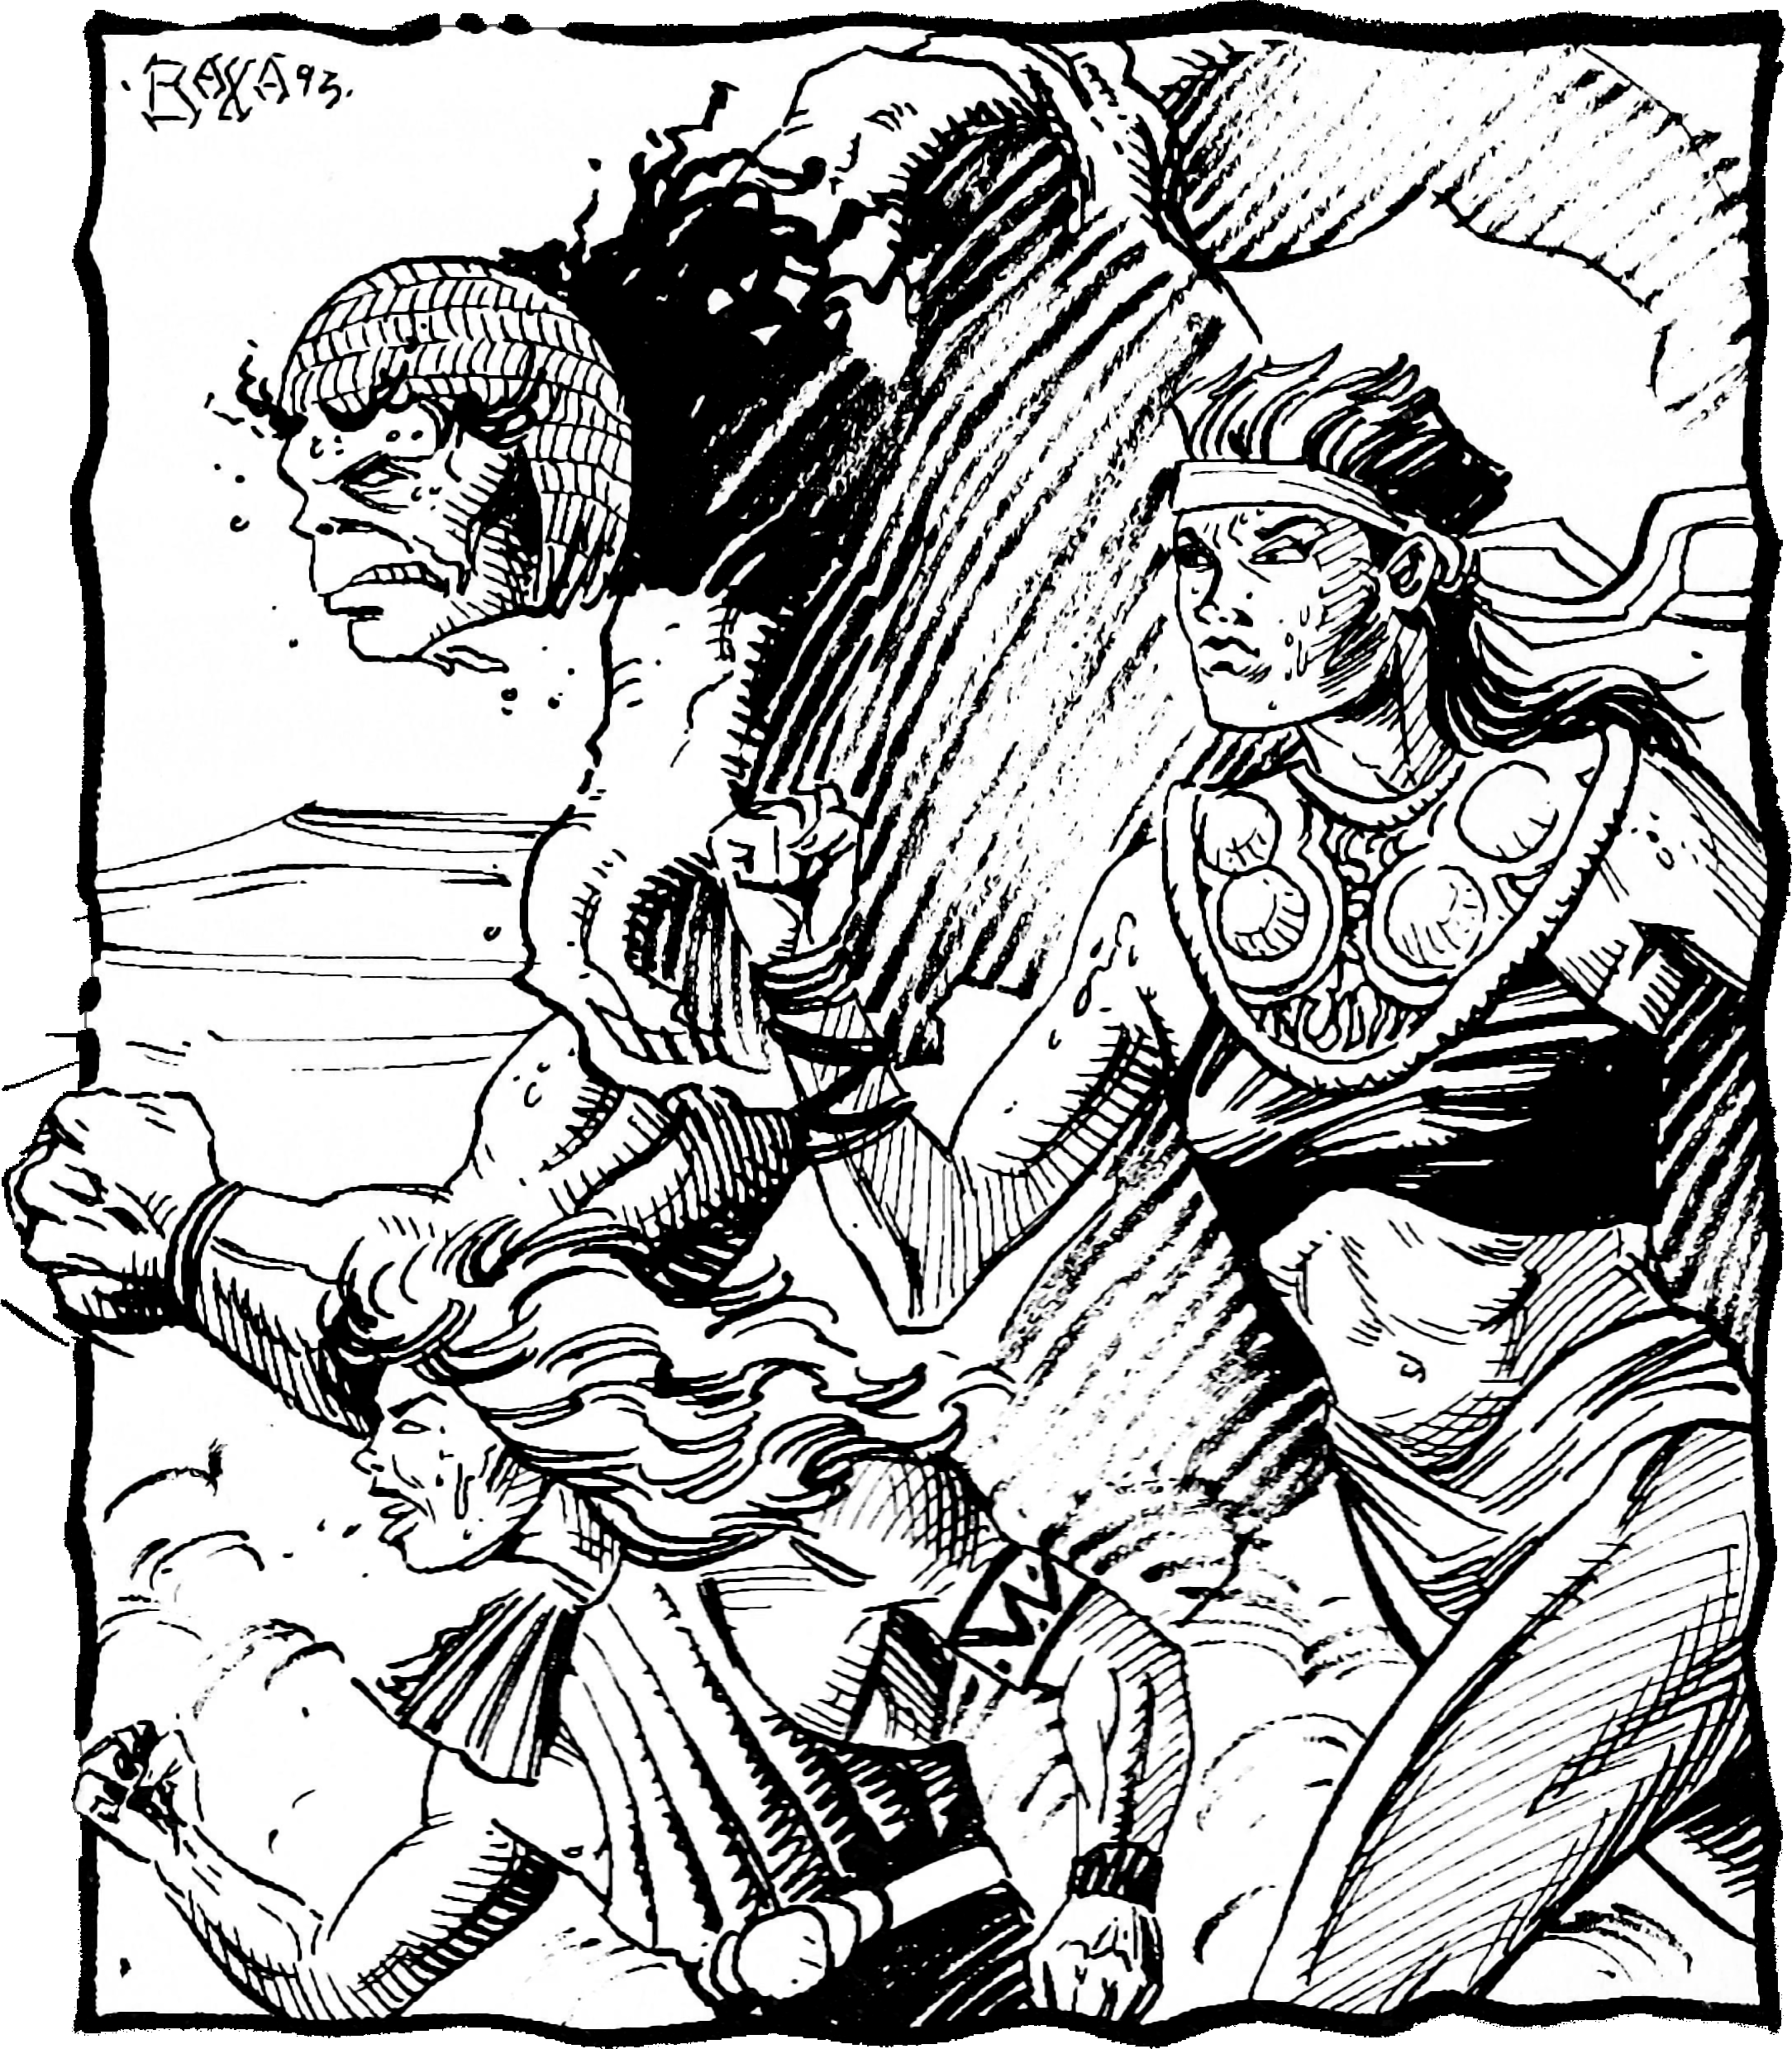
\includegraphics[width=\columnwidth]{images/running-1.png}
\WOTC
\end{figure}
\subsubsection{Run}
You can run as a full-round action. (If you do, you do not also get a 1.5-meter step.) When you run, you can move up to four times your speed in a straight line (or three times your speed if you're in heavy armor). You lose any Dexterity bonus to AC unless you have the \feat{Run} feat.

You can run for a number of rounds equal to your Constitution score, but after that you must make a DC 10 Constitution check to continue running. You must check again each round in which you continue to run, and the DC of this check increases by 1 for each check you have made. When you fail this check, you must stop running. A character who has run to his limit must rest for 1 minute (10 rounds) before running again. During a rest period, a character can move no faster than a normal move action.

You can't run across difficult terrain or if you can't see where you're going.

A run represents a speed of about 18 kilometers per hour for an unencumbered human.

\subsubsection{Move 1.5 meter through Difficult Terrain}
In some situations, your movement may be so hampered that you don't have sufficient speed even to move 1.5 meter (a single square). In such a case, you may spend a full-round action to move 1.5 meter (1 square) in any direction, even diagonally. Even though this looks like a 1.5-meter step, it's not, and thus it provokes attacks of opportunity normally.
\subsection{Free Actions}
\Table{Free Actions}{LZ{14mm}}{
\tableheader Action & \tableheader Attack of Opportunity\footnotemark[1] \\
Cease concentration on a spell & No \\
Drop an item & No \\
Drop to the floor & No \\
Prepare spell components to cast a spell\footnotemark[2] & No \\
Speak & No \\
\TableNote{2}{1 Regardless of the action, if you move out of a threatened square, you usually provoke an attack of opportunity. This column indicates whether the action itself, not moving, provokes an attack of opportunity.}\\
\TableNote{2}{2 Unless the component is an extremely large or awkward item.}\\
}

Free actions don't take any time at all, though there may be limits to the number of free actions you can perform in a turn. Free actions rarely incur attacks of opportunity. Some common free actions are described below.

\subsubsection{Drop an Item}
Dropping an item in your space or into an adjacent square is a free action.

\subsubsection{Drop Prone}
Dropping to a prone position in your space is a free action.

\subsubsection{Speak}
In general, speaking is a free action that you can perform even when it isn't your turn. Speaking more than few sentences is generally beyond the limit of a free action.

\subsubsection{Cease Concentration on Spell}
You can stop concentrating on an active spell as a free action.

\Table{Swift Actions}{LZ{14mm}}{
\tableheader Action & \tableheader Attack of Opportunity\footnotemark[1] \\
Assume stance & No \\
Cast quickened spell & No \\
Cast spell (1 swift action casting time) & No \\
Use gladiatorial performance & No \\
Use quickened spell-like ability & No \\
\TableNote{2}{1 Regardless of the action, if you move out of a threatened square, you usually provoke an attack of opportunity. This column indicates whether the action itself, not moving, provokes an attack of opportunity.}\\
}

\subsection{Swift Actions}
A swift action consumes a very small amount of time, but represents a larger expenditure of effort and energy than a free action. You can perform one swift action per turn without affecting your ability to perform other actions. In that regard, a swift action is like a free action. However, you can perform only a single swift action per turn, regardless of what other actions you take. You can take a swift action any time you would normally be allowed to take a free action. Swift actions usually involve spellcasting or the activation of magic items; many characters (especially those who don't cast spells) never have an opportunity to take a swift action.

Casting a quickened spell is a swift action. In addition, casting any spell with a casting time of 1 swift action is a swift action.

Casting a spell with a casting time of 1 swift action does not provoke attacks of opportunity.

\subsection{Immediate Actions}
\Table{Immediate Actions}{LZ{14mm}}{
  \tableheader Action
& \tableheader Attack of Opportunity\footnotemark[1] \\
Cast spell (1 immediate action casting time) & No \\
Use the \feat{Greater Counterspell} feat     & Yes \\
Use martial prowess                          & No \\
\TableNote{2}{1 Regardless of the action, if you move out of a threatened square, you usually provoke an attack of opportunity. This column indicates whether the action itself, not moving, provokes an attack of opportunity.}\\
}

Much like a swift action, an immediate action consumes a very small amount of time, but represents a larger expenditure of effort and energy than a free action. However, unlike a swift action, an immediate action can be performed at any time---even if it's not your turn. An immediate action is an instant response to a trigger of some kind. For example, an attack, a spell cast, a successful hit, or enemy reaching a specific spot.

Casting \spell{feather fall} is an immediate action, since the spell can be cast at any time.

Using an immediate action on your turn is the same as using a swift action, and counts as your swift action for that turn. You cannot use another immediate action or a swift action until after your next turn if you have used an immediate action when it is not currently your turn (effectively, using an immediate action before your turn is equivalent to using your swift action for the coming turn). You also cannot use an immediate action if you are flat-footed.

\vskip1cm
\subsection{Miscellaneous Actions}
\Table{Miscellaneous Actions}{LZ{14mm}}{
  \tableheader No Action
& \tableheader Attack of Opportunity\footnotemark[1] \\
1.5-meter step                                    & No \\
Delay                                             & No \\
Fight defensively                                 & No \\
Make \skill{Concentration} check                  & No \\
Make passive \skill{Listen} or \skill{Spot} check & No \\

% \cmidrule[0pt]{1-2}

  \tableheader Action Type Varies
& \tableheader Attack of Opportunity\footnotemark[1] \\
Disarm\footnotemark[2]           & Yes \\
Grapple\footnotemark[2]          & Yes \\
Trip an opponent\footnotemark[2] & Yes \\
Use feat\footnotemark[3]         & Varies \\

\TableNote{2}{1 Regardless of the action, if you move out of a threatened square, you usually provoke an attack of opportunity. This column indicates whether the action itself, not moving, provokes an attack of opportunity.}\\
\TableNote{2}{2 These attack forms substitute for a melee attack, not an action. As melee attacks, they can be used once in an attack or charge action, one or more times in a full attack action, or even as an attack of opportunity.}\\
\TableNote{2}{3 The description of a feat defines its effect.}\\
}

\subsubsection{Take 1.5-Meter Step}
You can move 1.5 meter in any round when you don't perform any other kind of movement. Taking this 1.5-meter step never provokes an attack of opportunity. You can't take more than one 1.5-meter step in a round, and you can't take a 1.5-meter step in the same round when you move any distance.

You can take a 1.5-meter step before, during, or after your other actions in the round.

You can only take a 1.5-meter step if your movement isn't hampered by difficult terrain or darkness. Any creature with a speed of 1.5 meter or less can't take a 1.5-meter step, since moving even 1.5 meter requires a move action for such a slow creature.

You may not take a 1.5-meter step using a form of movement for which you do not have a listed speed.

\subsubsection{Use Feat}
Certain feats let you take special actions in combat. Other feats do not require actions themselves, but they give you a bonus when attempting something you can already do. Some feats are not meant to be used within the framework of combat. The individual feat descriptions tell you what you need to know about them.

\subsubsection{Use Skill}
Most skill uses are standard actions, but some might be move actions, full-round actions, free actions, or something else entirely.

The individual skill descriptions tell you what sorts of actions are required to perform skills.

